\chapter{\Acl{la}} \label{chp:la}


\section{Introduction} \label{sec:la-intro}
\Gls{la} is a key technology to keep the \gls{bler} below a predefined threshold while maximizing the throughput.
%
The \gls{amc} is a key solution used in 4G systems and envisaged to \gls{5g} \gls{nr} system.
%
This approach consists in selecting the appropriate \gls{mcs} based on the channel quality.
%
% Basically, the systems use an \gls{amc} scheme that selects the appropriate \gls{mcs}.
% One key technique for \gls{la} is the \gls{amc} that selects the appropriate \gls{mcs}.
A very well known approach to perform such a selection is the use of \gls{amc}-like solutions.
%
They use the channel state information to keep the \gls{bler} below a predefined threshold.
% That is made based on the channel quality in order to keep the \gls{bler} below a predefined threshold.
%
In \gls{lte}, the target is fixed to 10\%, but the \gls{5g} \gls{nr} will cover a wider spectrum of services, and they impose new set of \gls{bler} targets \cite{Amin_2016,fantacci2009adaptive}.
%
Another aspect in \gls{la} is the rank adaptation, which defines the appropriate number of transmitted spatial streams is selected before transmission.
%
Rank adaptation is used in order to increase the throughput in low interference scenarios and reliability in high interference scenarios.

%
% \Gls{5g} wireless communication systems are being designed to provide high data and transmission rates \cite{Amin_2016}.
% %
% Because of this, a reliable link adaptation process for \gls{5g} \gls{nr} is needed for coping with the need of increasing the data rate that can be accurately transmitted \cite{chu01}.
% %
%
% In this context, the link adaptation technique of \gls{amc} is of great interest.
% %
% \Gls{amc} is a resource allocation technique used in link adaptation that allows the system to select the most appropriate \gls{mcs} to better cope with the changing channel conditions \cite{fantacci2009adaptive}.
% %

\Gls{amc} is a solution to match the modulation scheme and coding rate to the time-varying nature of the wireless channel.
%
Periodically, the \gls{ue} measures the channel quality and processes this information to map into a \gls{cqi}.
%
Typically, each \gls{cqi} represents a \gls{snr} interval \cite{Blanquez-Casado2016}.
%
The \gls{bs} uses the \gls{cqi} reported by the \gls{ue} to define the appropriate \gls{mcs}.
%
Thanks to the \gls{pdcch}, the new \gls{mcs} is informed to the \gls{ue} through the \gls{dci} \cite{ErikDahlman5G}.
%
By its turn, rank adaptation improves the systems performance, especially when used with \gls{irc} by selecting the number of transmission layers, or spatial multiplexing factor.
%
In high interference scenarios lower ranks are preferred as it improves the interference suppression at the receiver side and at low interference scenarios higher ranks can be used to increase the throughtput \cite{catania2015distributed}.
%
% In the downlink \gls{amc} procedure, the \gls{ue} suggests to the \gls{bs} an appropriate \gls{mcs} in the \gls{amc} set to be used \cite{Sang2014}.
% %
% This proposed \gls{mcs} is informed to the \gls{bs} by means of a \gls{cqi}, typically each \gls{cqi} represents a \gls{snr} interval \cite{Blanquez-Casado2016}.
% %
% In possession of this information, the \gls{bs} selects an \gls{mcs} to transmit and reports  its selection to the \gls{ue}.

\Gls{rl} framework has become an attractive tool to devise novel \gls{5g} \gls{la} due to the capacity of \gls{rl} tools in solving problems whose model varies over time.
%
% The goal of the \gls{la} is an automatic choice of the best parameters depending on the user, channel conditions and applications requirements.
% While in \gls{lte}, the look-up table provides fixed \gls{amc} rules for all the users, the novel system needs a more flexible one that can be adjusted according to user channel state.
%
\Gls{rl} falls into a category of \gls{ml} problems, and it has been applied in problems \cite{survey-son} such as backhaul optimization~\cite{jaber2015}, coverage and capacity optimization~\cite{Fan2014} and resource optimization~\cite{Miozzo2017SwitchOnOffPF}.
%
The use of RL in the context of LA has been recently addressed in \cite{continuousState}, \cite{bruno2014robust} and \cite{DRL_AMC}.

% The goal of the \gls{la} is an automatic choice of the best parameters, in this case the \gls{mcs}, depending on the user and applications requirements.
% %
% As such, \gls{ml} algorithms are well suited to this application, because of their capabilities of learning patterns, forecasting behaviors and generating models \cite{survey-son}.
%
% A \gls{ml} category of particular interest to cellular systems is the \gls{rl}, because of its applicability in optimization problems \cite{survey-son}, such as backhaul optimization~\cite{jaber2015}, coverage and capacity optimization~\cite{Fan2014} and resource optimization~\cite{Miozzo2017SwitchOnOffPF}.


% There are few works that use \gls{rl} in \gls{la} problem.
%
% In \cite{continuousState}, the selection of the \gls{mcs} is based on the received \gls{sinr}, as such the state space is continuous, and the learning algorithm must handle this large state space.
% %
% In \cite{bruno2014robust} a Q-learning approach is used to solve the \gls{amc} problem in the context of a \gls{lte} network.
%
% A deep reinforcement learning approach is used in \cite{DRL_AMC} as a solution to the \gls{amc} problem, in a cognitive heterogeneous network.
%

The main contributions of our work are:
\begin{enumerate}
    \item Proposition and analysis of a \gls{la} solution that selects the \gls{mcs} and the \gls{pmi} by using a \gls{rl} framework.
    \item Our solution complies with \gls{5g} \gls{nr} physical layer specification as we consider the whole chain of channel coding specified in the standard \cite{3gpp.38.212}
    \item It also complies with the \gls{5g} \gls{nr} procedures for data as it considers the multi-antenna precoder matrices from the standard \cite{3gpp.38.214}.
\end{enumerate}
%
Furthermore, our solution complies with \gls{5g} \gls{nr} physical layer specification as we consider the whole chain of channel coding specified in the standard \cite{3gpp.38.212} while also using the multi-antenna precoder matrices from the standard \cite{3gpp.38.214}.
% As such, the main difference between our work and the previous approaches is the implementation of the channel coding as proposed by the \gls{5g} standard while also using the multi-antenna precoder matrices from the standard \cite{3gpp.38.214}

%%%%%%%%%%%%%%%%%%%%%%%%%%%--End Of Section--%%%%%%%%%%%%%%%%%%%%%%%%%%%%%%%

\section{System Model}
\label{sec:la-system-model}
%\subsection{Signal Model}

Consider a single cell system whose \gls{bs} is equipped with \gls{not:txAnt} antennas serving one user equipped with \gls{not:rxAnt} antennas.
%
Let us assume a transmission mode with a multilayer scheme, where the \gls{bs} uses a precoder \gls{not:Wtx} \inSetComplex{\gls{not:txAnt}}{\gls{not:nLayers}} to transmit data over  \gls{not:nLayers} layers, while the \ue~applies a \gls{mmse} filter \gls{not:Wrx} \inSetComplex{\gls{not:nLayers}}{\gls{not:rxAnt}}.
%
The discrete received signal model at the receiver is represented as
\begin{equation}
\label{eq.:rx_signal}
\gls{not:Y} =
\gls{not:Wrx}
\channel
\gls{not:Wtx}
\gls{not:sscl}
% _\userIdx
+
\gls{not:Wrx}
\gls{not:Z} \;,
\end{equation}
\noindent where $\channel $ \inSetComplex{\gls{not:rxAnt}}{\gls{not:txAnt}} represents the channel between the \bs~ and the \ue, $\gls{not:sscl}$ represents the transmitted symbols at each layer to the \ue, and \gls{not:Z} is the Gaussian noise with zero mean and variance \gls{not:var}.
%
The filter \gls{not:Wrx} is calculated from the channel perceived by the receiver, $\channel_{\textrm{rx}} = \channel \gls{not:Wtx}$, as:

\begin{equation}
\label{eq.:Wrx}
\gls{not:Wrx} =
(
\channel_{\textrm{rx}}^H
\channel_{\textrm{rx}}
+
\frac{ \gls{not:var} }{ p_{\gls{not:sscl}} }
\mathbf{I}_{\gls{not:nLayers}} )^\dagger
\channel_{\textrm{rx}}^H \;,
\end{equation}

\noindent where the operator $\dagger$ represents the Moore-Penrose inverse, $\mathbf{ I}_{\gls{not:nLayers}} $ is the $\gls{not:nLayers} \times \gls{not:nLayers}$ identity matrix and $p_{\gls{not:sscl}}$ is the the power of the transmitted signal \gls{not:sscl}.
%
We define the \gls{snr} of the stream $i$ as:
%
\begin{equation}
\label{eq.:snr}
\textrm{SNR}_i = \frac{ \abs{
		% \hermitian{\gls{not:Wrx}\subArg{\userIdx}\argPair{:}{\idxI}}
		\channel_{\textrm{eq}} (i,i)
		% \subArg{\userIdx} \gls{not:Wtx}\subArg{\userIdx}\argPair{:}{\idxJ}
	}^2 }{\gls{not:var}_{eq}} p_{\gls{not:sscl}} \; ,
\end{equation}
%
where $\channel_{\textrm{eq}} = \gls{not:Wrx} \channel \gls{not:Wtx}$ and the $\gls{not:var}_{\textrm{eq}}$ is given by:
%
\begin{equation}
\gls{not:var}_{\textrm{eq}} = \frac{
	\Tr \,  (\abs{ \gls{not:Wrx}^H \gls{not:Wrx} } )}
{\gls{not:rxAnt}}
\gls{not:var} \;.
\end{equation}
% \subsection{Channel Description}


The model in \eqref{eq.:rx_signal} assumes a narrowband block-fading channel, so the channel is almost constant within a time-frequency resource block \cite{alkhateeb2014}.
%
We assume a geometric channel model with a limited number \gls{not:scatterers} of scatterers.
%
Each scatterer contributes with a single path between \gls{bs} and \gls{ue}. Therefore, the channel model can be expressed as
%
\begin{equation}\label{eq.:channelModel}
\channel = \sqrt{\pathloss}\sum_{k=0}^{\gls{not:scatterers} - 1 }\gls{not:beta}_k \strRx \anglePair{k}{UE} \hermitian{\strTx  \anglePair{k}{\textrm{UE}}},
\end{equation}
\noindent where $\pathloss$ denotes the pathloss, \gls{not:beta} is the complex gain of the $k$th path.
%
The azimuth \azm~$\in$ \range{0}{2\pi} and the elevation \elev~$\in$ \range{0}{\pi} are the \gls{aod} and \gls{aoa} at the \bs~and \ue , respectively.
%
We assume a \glspl{ura} at the \gls{bs} and \gls{ue}. There are $\gls{not:txAnt}_{v}$ vertical antenna elements and  $\gls{not:txAnt}_{h}$ horizontal antennas elements, such that $\gls{not:txAnt} = \gls{not:txAnt}_{v} \gls{not:txAnt}_{h}$. The array response at the \gls{bs} is expressed as
%
% \begin{dmath}
% 	\strTx \anglePair{k} = \frac{1}{\sqrt{\gls{not:txAnt}}}\left[1, \ldots ,\expUraPhase{(\gls{not:txAnt} -1 )}{k} \right],
% \end{dmath}
% where \dist ~is the antenna element spacing, and \wave~is the signal wavelength. The array response at \gls{ue} can be written similarly.
\begin{equation}
\begin{split}
\strTx \anglePair{k}{BS} = \frac{1}{\sqrt{\gls{not:txAnt}}}\left[1, \ldots , e^{\jmath  \left( (\gls{not:txAnt}_{v} - 1)\frac{2\pi \Delta}{\lambda} (\cos{\elev_{k}^{\textrm{\tiny{(BS)}}}}) + (\gls{not:txAnt}_{h} - 1)\frac{2\pi \Delta}{\lambda}\left (\sin{\azm_{k}^{ \textrm{\tiny{(BS)}} }} \sin{\elev_{k}^{\textrm{\tiny{(BS)}} }} \right)   \right)}  \right]^{T},
\end{split}
\end{equation}
where $\Delta$ ~is the antenna element spacing, and \wave~is the signal wavelength. The array response at \gls{ue} can be written similarly.

The \gls{mimo} channel in \eqref{eq.:channelModel} can be expressed compactly as
\begin{equation}
\label{eq.:channelModelMtx}
\channel  = \strRxMtx \diag{\gls{not:betaVec}} \hermitian{\strTxMtx},
\end{equation}
where $\gls{not:betaVec} = \left[ \gls{not:beta}_0, \ldots, \gls{not:beta}_{\gls{not:scatterers}-1} \right]$, and the matrices \strRxMtx~and \strTxMtx~are formed by the concatenation \gls{ue} and \gls{bs} array response vectors, respectively.

%\subsection{Transmission Model}

% The transmission process takes into account the channel coding, modulation, layer mapping and multi-antenna precoding blocks of Figure \ref{fig:transmission}.
%
In this work, we implement \gls{phy}/\gls{mac} layer as specified in \cite{3gpp.38.212} and depicted in Figure \ref{fig:transmission}.
%
%In this study we implemented all the steps specified in the channel coding block.
%
The \gls{tbs} calculation, the \gls{mcs} tables and the multi-antenna precoding matrices, \gls{not:Wtx}, follow the specifications in \cite{3gpp.38.214}.
%


% The \gls{ue} reports the measured \gls{cqi} to the \gls{bs}, which decides the \gls{mcs} and \gls{pmi} accordingly.
The \gls{cqi} plays an important role to properly select the \gls{mcs} and \gls{pmi}.
%
The \gls{mcs} and \gls{ri} are informed to the \gls{ue} through the \gls{pdcch} as a part of the \gls{dci}. This process is shown in Figure \ref{fig:la-system-model}.
%
The \gls{cqi} is a measure of the \gls{snr}, and the number of possible \gls{cqi}s is defined by $n_{cqis}$. We define the \gls{cqi} as:
% \begin{equation}\label{eq:cqi}
%     CQI =
%     \begin{cases}
%     0, \text{if } SNR \leq SNR_{min}\\
%     (N_{cqi}-1), \text{if } SNR \geq SNR_{max}\\
%     \floor[\Big]{\frac{(SNR - SNR_{min})(n_{cqis}-1)}{SNR_{max}-SNR_{min}}},
%     \end{cases}
% \end{equation}
\begin{equation}\label{eq:cqi}
\textrm{CQI} = \min{
	(\max {(0, \textrm{CQI}^{\prime} ) }, n_{cqis} - 1)},
\end{equation}

\noindent where $\textrm{CQI}^{\prime}$ is calculated from the \gls{snr}s in dB as:
\begin{equation}\label{eq:cqi_prime}
\textrm{CQI}^{\prime} = \floor[\Big]{(n_{cqis}-1)\frac{\textrm{SNR} - \textrm{SNR}_{min}}{\textrm{SNR}_{max}-\textrm{SNR}_{min}}}
\end{equation}

% \noindent note that each \gls{cqi}, except the minimum and the maximum, comprises \gls{snr} intervals having the same length in dB.
% , since the \gls{snr} inside the range $[snr_{min},snr_{max}]$ is divided equally into \gls{cqi}s in this calculation.

At each \gls{tti}, the \gls{bs} calculates the \gls{tbs}, taking into account the selected \gls{mcs} and the number of spatial layers, and transmits a \gls{tb} with \gls{tbs} bits at the chosen \gls{mcs} and using the selected multi-antenna precoding matrix from the \gls{pmi}.
%
The \gls{ue} receives a \gls{tb} from the \gls{bs} and, in possession of the chosen \gls{mcs}, decodes the \gls{tb} and calculates its \gls{crc}, giving the \gls{bs} a \gls{acknack} that is further used to calculate the \gls{tbler} and the throughput.
%
The \gls{tbler} is the ratio of incorrectly received \gls{tb}s over the total number of transmitted \gls{tb}s.

\begin{figure}[!hb]
	\centerline{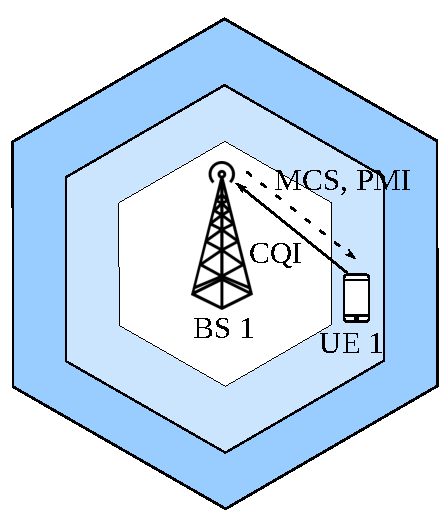
\includegraphics[width=50mm]{figures/chp_la/system-model-mateus.pdf}}
	\caption{Exchange of signals referent to the link adaptation}
	\label{fig:la-system-model}
\end{figure}

%%%%%%%%%%%%%%%%%%%%%%%%%%%%%%%%%%--End Of Section--%%%%%%%%%%%%%%%%%%%%%%%%%%%%%%%%%%%%%

\section{Proposed Solution}
\label{sec:la-proposed}

The proposed solution is a Q-learning based \gls{la} scheme, herein referred to as \gls{ql-la}.
%
The \gls{bs} uses two \gls{rl} agents, one to select the \gls{mcs} and another to select the \gls{pmi}.
%
Both selections are based on the state-action mapping obtained from the two Q-learning algorithms.
%
The \gls{rl} based solution enables the system to learn the particularities of the environment and adapt to it.


% The choice of using two agents in the \gls{bs} is due to the large action space if a single agent chooses both the \gls{mcs} and \gls{pmi}, hence a multi-agent approach leads to a faster learning since less samples are required to fill up the Q-tables.
The use of two agents is motivated by the reduced computational complexity to compute the action-state space.
%
While using a single agent requires a large Q-table to construct all the possible \gls{mcs} and \gls{pmi} combinations, multiple agents solve the problem separately by computing two smaller Q-tables.
% More specifically, the \gls{bs} chooses the \gls{mcs} and the \gls{pmi} using the Q-tables obtained from the \gls{rl} algorithms.
%
Figure \ref{fig:la-rl-frame} shows how the \gls{rl} framework fits the \gls{la} problem.

% A diagram adapting the model from Figure \ref{fig:rlbasic} to the \gls{la} problem is shown in Figure \ref{fig:rl-frame}.
%
\begin{figure}[!hb]
	\centerline{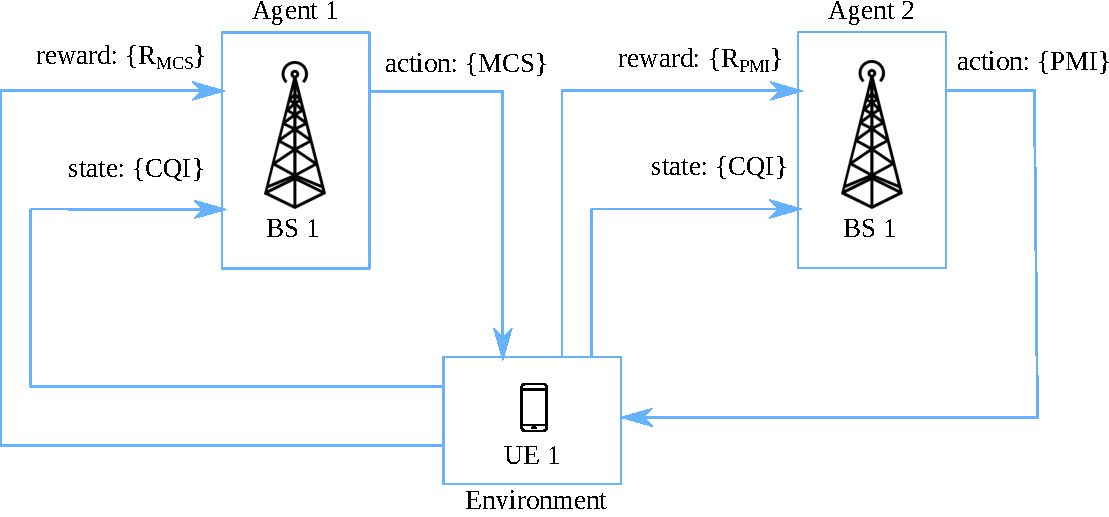
\includegraphics[height=60mm]{figures/chp_la/rl-framework-mateus.pdf}}
	\caption{Basic diagram of the proposed AMC scheme}
	\label{fig:la-rl-frame}
\end{figure}
%

In the proposed \gls{la} solution, the state space is the set of all possible \gls{cqi}s, from $0$ to $(n_{cqi}-1)$, for both agents; the action space is the set of all possible \gls{mcs}s for the agent 1 and the set of all possible \gls{pmi}s for the agent 2. As for the reward for each agent, $R_{PMI}$ is defined as:
%
\begin{equation}\label{eq.:rewardPMI}
R_{PMI} = \begin{cases}
\gls{not:nLayers}, \text{ if ACK} \\
0, \text{ else,}
\end{cases}
\end{equation}
%
\noindent where \gls{not:nLayers} is the number of transmission layers. The $R_{MCS}$ is defined as:
\begin{equation}\label{eq.:rewardMCS}
R_{MCS} = \begin{cases}
\dfrac{\textrm{\gls{tbs}}}{\gls{not:nLayers}}, \text{ if ACK} \\
0, \text{ else,}
\end{cases}
\end{equation}
\noindent where \gls{tbs} is the number of transmitted information bits and is defined in terms of \gls{not:nLayers} as shown in \cite{3gpp.38.214}.
%
The division of \gls{tbs} by \gls{not:nLayers} in Eq. \eqref{eq.:rewardMCS} is used to make the reward of the \gls{mcs} agent more independent from the \gls{pmi} choice.
% The \gls{tbs} calculation is defined in \cite{3gpp.38.214} and it is dependent of the \gls{not:nLayers}, hence the division is used to make the reward of the \gls{mcs} agent more independent from the \gls{pmi} choice.
%

% \begin{table}[!hb]
% \centering
% \caption{\gls{rl} elements}
% \label{tab:ql-amc-def}
% \begin{tabularx}{0.5\columnwidth}{X r}
% \toprule
% \textbf{Element} 	      & \textbf{Definition} \\
% \midrule
% State                   & \gls{cqi} \\
% Action                  & \gls{mcs} \\
% % Reward                  & Eq: \eqref{eq.:reward1}, \eqref{eq.:reward2}, \eqref{eq.:reward3} \\
% \bottomrule
% \end{tabularx}
% \end{table}
% %



%%%%%%%%%%%%%%%%%%%%%%%%%%%%%%%%%%--End Of Section--%%%%%%%%%%%%%%%%%%%%%%%%%%%%%%%%%%%%%

\section{Simulations and Results}
\label{sec:la-simulation}
\subsection{Simulation Parameters}
We assess the system performance with one \gls{bs} that serves one \gls{ue}.
%
The system has a bandwidth $B$ with a frequency carrier of $28$ GHz.
%
Each resource block has a total of $12$ subcarriers and a subcarrier spacing $\gls{not:sub-spacing} = 120 \text{KHz}$ .
%
A \gls{nr} frame is composed by 10 subframes, and each one consists of multiple slots, where each slot has 14 symbols.
%
We consider the channel model defined in \eqref{eq.:channelModel}.
%
The path loss is a urban macro (UMa) with non-line-of-sight (NLOS), and the shadowing is modeled as a log-normal distribution with standard deviation of $6$ dB \cite{AliZaidi632018}.
%
The noise power is modeled as $10\log_{10}(290 \cdot 1.38 \cdot 10^{-23} \cdot \Delta f \cdot 10^3 )$ dBm.
%

Tables~\ref{tab:la-sim-params} and \ref{tab:la-rl-params} list the simulation and \gls{ql-la} parameters.

% The main simulation parameters are listed in Table~\ref{tab:sim-params} and the parameters selected for the \gls{ql-la} are listed in Table \ref{tab:rl-params}.
Several combinations of the Q-Learning parameters $\alpha$ and $\gamma$ were tested and the combination that gives the best average throughput was kept.


\begin{table}[!htb]
	\centering
	\caption{General  Simulation Parameters}
	\label{tab:la-sim-params}
	\begin{tabularx}{0.7\columnwidth}{X r}
		\toprule
		\textbf{Parameter} 	& \textbf{Value} \\
		\midrule
		Min. dist. \gls{bs}-\gls{ue} (2D) & 35 m\\
		\gls{bs} height & 15 m\\
		\gls{ue} height & 1.5 m\\
		\gls{ue} track & linear\\
		\gls{bs}  antenna model & omnidirectional \\
		\gls{bs}  antennas & 2 \\
		\gls{ue} antenna model & omnidirectional \\
		\gls{ue} antennas & 4 \\
		Transmit power & 42 dBm\\
		Frequency & 28 GHz\\
		Bandwidth & 1440 MHz\\
		Number of subcarriers  & 12\\
		Subcarrier spacing & 120 kHz\\
		Number of subframes & 10\\
		Number of symbols & 14\\
		Azimuth angle range & $[-60^{\circ}, 60^{\circ}]$\\
		Elevation angle range & $[60^{\circ}, 120^{\circ}]$\\
		% Number of paths & 10\\
		Path loss & UMa NLOS\\
		Shadowing standard deviation & 6 dB\\
		%Noise spectral density & -123 & dBm/Hz\\
		\bottomrule
	\end{tabularx}
\end{table}



\begin{table}[!htb]
	\centering
	\caption{Reinforcement Learning Parameters}
	\label{tab:la-rl-params}
	\begin{tabularx}{0.6\columnwidth}{X r}
		\toprule
		\textbf{Parameter} 	 & \textbf{Value} \\
		\midrule
		Discount factor ($\gamma$)  & 0.50\\
		Learning rate ($\alpha$) & 0.70\\
		Maximum exploration rate ($\epsilon_{\max}$) & 0.50\\
		Minimum exploration rate ($\epsilon_{\min}$) & 0.05\\
		$n_{cqis}$ & 16 \\
		\bottomrule
	\end{tabularx}
\end{table}

\subsection{Baseline Solutions}

We assume as baseline solution a fixed lookup table scheme and a multi-antenna precoder selection that leads to maximum mean \gls{snr} defined in Eq. \eqref{eq.:snr}.

% We compare the \gls{ql-la} against a baseline solution, in which the \gls{mcs} selection is based on a \gls{amc} with a fixed look-up table \cite{fantacci2009adaptive} selection and it selects the multi-antenna precoder that results in the maximum mean \gls{snr} in Eq. \eqref{eq.:snr}.
%
In the fixed look-up table approach, a static mapping of the \gls{snr} to \gls{cqi} is obtained by analyzing the \gls{bler} curves and selecting the best \gls{mcs}, in terms of throughput, that satisfies the target \gls{bler} \cite{bruno2014robust}.
%
The process of analyzing the \gls{bler} curves gives the \gls{snr} thresholds that separate each \gls{cqi}.
%
We assumed a direct mapping of the \gls{cqi} to \gls{mcs}, i.e., each \gls{cqi} is mapped to one \gls{mcs}.
%
% Table \ref{tab:lookup} shows the \gls{cqi} to \gls{mcs} mapping, for a target \gls{bler} of $0.1$.
% %
% This table was obtained by analyzing the \gls{bler} curves in a \gls{awgn} channel.
%
% \begin{table}[!htb]
% \centering
% \caption{Lookup Table}
% \label{tab:lookup}
% \begin{tabularx}{0.4\columnwidth}{X X r}
% \toprule
%  CQI   & Modulation   & Rate \\
% \midrule
%  0     & QPSK         & 1/3   \\
%  1     & QPSK         & 1/2   \\
%  2     & QPSK         & 2/3   \\
%  3     & 16QAM        & 1/2   \\
%  4     & 16QAM        & 2/3   \\
%  5     & 16QAM        & 3/4   \\
%  6     & 64QAM        & 2/3   \\
%  7     & 64QAM        & 3/4   \\
%  8     & 64QAM        & 5/6   \\
% \bottomrule
% \end{tabularx}
% \end{table}

\subsection{Experiment Description and Results}

% The experiment devised to assess the performance of the \gls{ql-la} in comparison to the baseline is composed of two phases, namely the training phase and deployment phase.
Our simulation has two phases: the training phase and the deployment phase. We use the first phase to train the agents to learn the environment dynamics while the second phase we use the knowledge acquired to make decisions, while comparing to the baseline.

\subsubsection{Training Phase}
% In the first phase, the \gls{rl} agents populates the Q-table to understand the environment.
%

Our simulation initializes with the \gls{ue} at a position with a radial distance of $35m$ of the \gls{bs} and goes away from the \gls{bs} in the opposite direction.
%
Then the \gls{ue} comes back to the center after reaching $180m$ from the \gls{bs}, and then it moves away again from the \gls{bs} to $180m$.
%
The simulation runs for a equivalent of $80s$ with the \gls{ue} speed equal to $20m/s$, this is equivalent to 8000 frames.
%
At the beginning of the transmission time, the channel has 10 paths and it changes after every $5m$ traveled, being either 1 (e.g. to emulate an environment change to LOS) or 10.

%
We use \gls{ql-la} with three configurations, as follows:
\begin{enumerate}
    \item the precoding/beamforming vector is selected by fixing the transmission rank to one;
    \item the precoding/beamforming matrix is selected by fixing the transmission rank to two;
    \item both the precoding/beamforming structure and the transmission rank are adapted.
\end{enumerate}
% We analyzed three \gls{ql-la} configurations, with a fixed transmission rank of one and two, therefore only selecting the \gls{pmi}s for these ranks, and a adaptive rank solution.
%
Table \ref{tab:la-train-results} summarizes the results, providing  an average value of the throughput  and the \gls{tbler}.
%
\begin{table}[!htb]
	\centering
	\caption{Training Phase Results}
	\label{tab:la-train-results}
	\begin{tabularx}{0.6\columnwidth}{X X r}
		\toprule
		Solution        &   TBLER   & Throughput    \\
		\midrule
		Adaptive        &   0.1814  & 3.8644        \\
		Single Stream   &   0.0932  & 4.1581        \\
		Dual Stream     &   0.5128  & 1.5963        \\
		\bottomrule
	\end{tabularx}
\end{table}

Table \ref{tab:la-train-results} reveals that the \gls{ql-la} with only a single stream (i,.e. rank-one transmission) shows a better performance in terms of throughput and \gls{tbler}, while the dual stream solution has a poor \gls{tbler} and throughput.
%
Figure \ref{fig:la-train-thr} shows the throughput averaged over a sliding window of 400 transmissions, during a total transmission time of 80 sec.

\begin{figure}[!htbp]
	\centerline{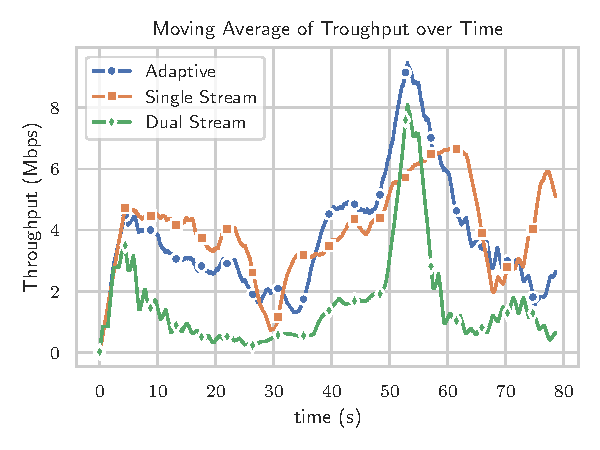
\includegraphics[width=0.6\columnwidth]{figures/chp_la/Thr_Train.pdf}}
	\caption{Moving average of throughput on training phase}
	\label{fig:la-train-thr}
\end{figure}

% \begin{figure}[!htbp]
% \centerline{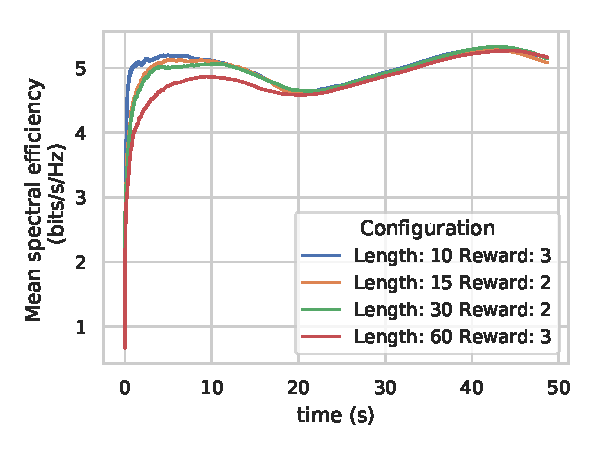
\includegraphics[width=0.7\columnwidth]{figures/Spec-Eff-Train.pdf}}
% \caption{Mean spectral efficiency on training phase}
% \label{fig:train-spceff}
% \end{figure}
%
% \begin{figure}[!htbp]
% \centerline{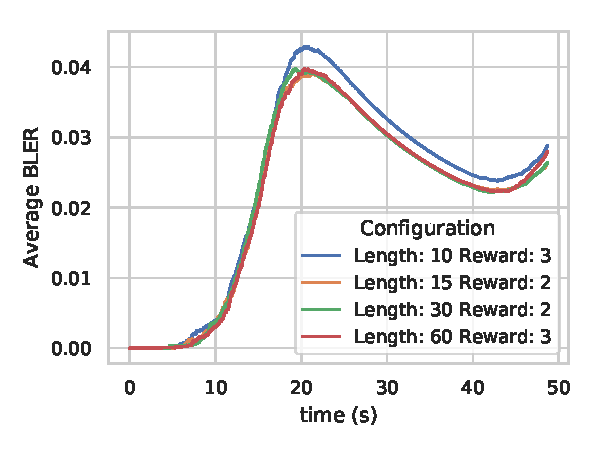
\includegraphics[width=0.7\columnwidth]{figures/BLER-Train.pdf}}
% \caption{Mean \gls{bler} on training phase}
% \label{fig:train-bler}
% \end{figure}


Figure \ref{fig:la-train-thr} shows that the dual stream solution provides a high peak rate, but also presents the worse overall performance during most of the time, compared to the other solutions.
%
The rank-adaptive solution offers the higher rates during a time window (between 40 and 55 s).
%
Note that the rank-adaptive \gls{ql-la} scheme outperforms the dual stream scheme, and is worse than the single stream scheme for some transmission intervals.
%
This result is probably due to the fact that, during the exploration phase, the rank-adaptive scheme sometimes attempts a dual stream transmission whereas the right choice would be a single stream one.

\subsubsection{Deployment phase}
The second phase uses the knowledge from the first phase, but with a $\epsilon$-greedy approach with a fixed value of $\epsilon = 0.05$, according to the minimum value of the $\epsilon$-decreasing in the training phase.
%
The goal is to have an assessment of how the \gls{rl} solution performs in the long run, in contrast to the first phase (Figure \ref{fig:la-train-thr}) that focus on the learning of the agents.
%

In this phase, we compare the \gls{ql-la} with the baseline solution.
%
We perform $200$ Monte Carlo runs. At each run, the \gls{ue} starts at a random position between $35m$ and $140m$ of the \gls{bs}.
%
The \gls{ue} moves in a random rectilinear direction with a random speed between $10km/h$ and $20km/h$. Each simulation for a transmission time equivalent to $100ms$ which corresponds to 10 frames.
%
Similar for the previous experiment, at the beginning of the transmission time, the channel has 10 paths.
%
In the middle of the transmission time, the channel rank drops to 1 to emulate an environment change to LOS.
%

Table \ref{tab:la-deploy-results} shows the throughput and the \gls{tbler} of each \gls{ql-la} solution as well as the performance of the baseline solution..
%
\begin{table}[!htb]
	\centering
	\caption{Deployment Phase Results}
	\label{tab:la-deploy-results}
	\begin{tabularx}{0.6\columnwidth}{X X r}
		\toprule
		Solution        &   TBLER   & Throughput    \\
		\midrule
		Adaptive        &   0.0348  & 5.3012       \\
		Single Stream   &   0.0129  & 5.6952        \\
		Dual Stream     &   0.1075  & 4.4761        \\
        Baseline        &   0.0539 &  5.9712        \\
		\bottomrule
	\end{tabularx}
\end{table}
%
The results reveal that the proposed single-stream and rank-adaptive \gls{ql-la} schemes yield a better performance in terms of \gls{tbler}, while baseline solution shows a higher throughput.
%
Figure \ref{fig:la-deploy-thr} summarizes the results in the deployment phase.
%in terms of average values for each configuration of the \gls{ql-la} and baseline solution.
%
\begin{figure}[!htbp]
	\centerline{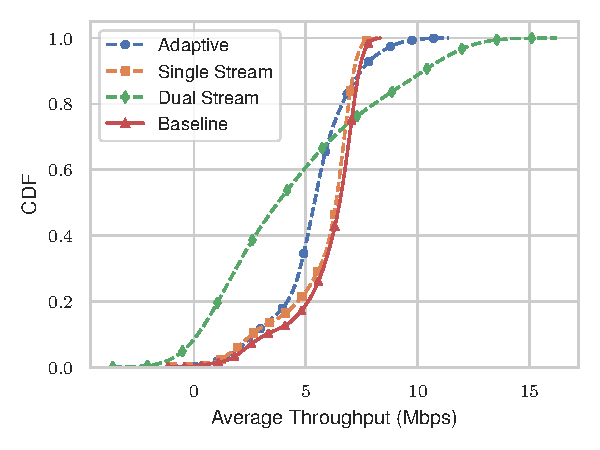
\includegraphics[width=0.6\columnwidth]{figures/chp_la/Thr_LA.pdf}}
	\caption{CDF of the average throughput (Mbps)}
	\label{fig:la-deploy-thr}
\end{figure}

We can note that the single stream \gls{ql-la} has a similar performance to the baseline solution, while the rank-adaptive \gls{ql-la} presents a slightly worse performance..

%%%%%%%%%%%%%%%%%%%%%%%%%%%%%%%%%%--End Of Section--%%%%%%%%%%%%%%%%%%%%%%%%%%%%%%%%%%%%%


\section{Conclusions and Perspectives}
\label{sec:la-conclusion}
The \gls{rl} provides a self-exploratory framework that enables the \bs~ to choose a suitable \gls{mcs} and multi-antenna precoding matrix that maximizes the throughput.
%
% Basically, the \gls{bs} decides a specific \gls{mcs} and \gls{pmi} at a certain time instant. And the \gls{bs}, in possession of the \gls{acknack} of the \gls{ue} calculates the performance of each agent.
%
In comparison to the baseline solution, consisting of a genie-aided precoder selection and a \gls{mcs} lookup table, our single stream \gls{ql-la} scheme has a similar performance, while the rank-adaptive \gls{ql-la} presents a slightly worse performance.
%
We believe this result was due to a simulation setting that favors single stream transmission.
%
A fine-tuning of our multi-agent \gls{ql-la} is being studied and may improve the result of the rank-adaptive approach.
%
This is a topic that is under investigation.

As a perspective of this work, we highlight the extension of the proposed \gls{rl}-based framework to include all the precoders of the standard \cite{3gpp.38.214} and the evaluation of a single \gls{rl} agent choosing both the \gls{mcs} and the \gls{pmi}.
%
Moreover, a comparison with other \gls{rl}-based algorithms such as multi-armed bandits (MABs) \cite{zhou2015survey} or deep RL solutions \cite{DeepRLSurvey} is envisioned.
%
% In addition, since \gls{nr} is a beam-based system, including the beam domain is another perspective.
% %
% In other words, our \gls{rl}-based solutions can also incorporate the selection of the best beam to transmit/receive data, among a set of choices (codebook).
% %
% These perspectives will be addressed in a follow-up work.
